% !TeX encoding = UTF-8
% !TeX spellcheck = es_ES
% !TeX root = Esquema.tex
% !TEX root = Esquema.tex


\section{Sectores}
Los sectores son las diferentes agrupaciones en las que se divide la maqueta desde unos punto de vista electricos. Los fabricantes suelen llamar a cada una de elementos agruados como \textbf{Districtos} y \textbf{Bloques} \sidenote{Solo para Digital}.

La principal caracterisitica de cada elemento es que esta aislado electricamente del resto\sidenote{En maquetas DC o Analogicas, son conceptos paralelos a cada circutito que puede ser controlado por un mando}. Cada uno de estos elementos (distritos o bloques) va estar precedido por un aparato que conecte dicho elemento a la fuente de energia DCC\sidenote{Ya sea un booster o una central}. La diferencia radica en el objetivo que se quiere obtener con la segmentacion y por lo tanto el dispositivo a conectar. 

\begin{itemize}
\item \textbf{Bloque}: tambien llamado \textit{<<Bloque de deteccion>>}, monitoriza el consumo de corriente y con esa informacion puede inferir si el bloque esta ocupado. 

Puede incluir un detector/lector RailComm y asi poder obtener informacion de la maquina/decoder que esta ocupando el bloque y enviandola al bus LCB.

El bloque debe ser lo más pequeño posible para que solo pueda entrar un elemento a detectar, pero lo suficientemente grande como para detectar el material más grande que se quiera detectar.

\item \textbf{Districto Electrico}: Protege al resto de \textit{districtos} de corto circuitos que puedan exitir en la seccion protegida. El dispositivo conectado controla que el consumo en un   \textit{districto} no supere un cierto umbral, a partir del cual considera que hay un corto y desconecta el distrito de la fuente de potencia.

Hoy en dia las centrales y los booster tienen protecciones ante corto, por lo tanto podria parecer que la division en distritos no es necesaria. Pero si no existen esta particion, un corto, como por ejemplo en la playa de vias, provocaria que toda la maqueta se parara, mientras que con los districtos, en el ejemplo, solo la playa estara sin energia y el resto de la maqueta seguiria funcionando.
\end{itemize}


La maqueta se ha realizado por secciones delimitadas por lo tableros, as 


\begin{figure}[H]
    \centering
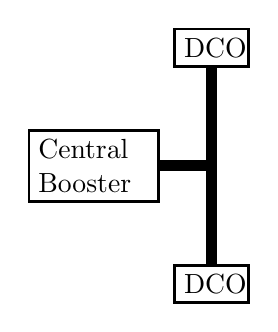
\begin{tikzpicture}

    %\draw [very thin, green]  (-6,-3) grid (6,3);
	\paintBoard 

	\paintStation[BlueGreen!25]{5pt}
	\paintStation[gray]{2pt}
   \paintTerminus[gray]{2pt}
   
	\paintYard[BrickRed!25]{5pt}
	\paintYard[gray]{2pt}
	  
	\paintMain[gray]{2pt}

	\node[draw=black, text width=4em, line width=1pt](central) at (-8.5,0) {Central Booster};

	\node[draw=black, text width=2em, line width=1pt] (dco1) at (-7,1.5) {DCO};

	\node[draw=black, text width=2em, line width=1pt] (dco2) at (-7,-1.5) {DCO};
	\draw[line width=4pt] (central.east) -- (-7,0)
	-- (dco1.south) -- (dco2.north);
	
\end{tikzpicture}

    \caption{Zonas de la maqueta}
    \label{fig:particion}
\end{figure}
